\usepackage{booktabs}
\usepackage{longtable}
\usepackage{float}
\usepackage[bf,singlelinecheck=off]{caption}
\usepackage[justification=centering]{caption}
\usepackage{fancyhdr}
\usepackage{fontspec}
\usepackage{color}
\usepackage{titling}

% changer la taille des en-tetes
\fancyhead{}
\fancyfoot{}
\renewcommand{\headrulewidth}{0pt}
\fancyhead[RO,LE]{\footnotesize\thepage}
\fancyhead[RE]{\footnotesize\slshape\leftmark}
\pagestyle{fancy}

\usepackage{framed,color}
\definecolor{shadecolor}{RGB}{248,248,248}
\definecolor{shadebluecolor}{RGB}{224,244,255}

\renewcommand{\textfraction}{0.05}
\renewcommand{\topfraction}{0.8}
\renewcommand{\bottomfraction}{0.8}
\renewcommand{\floatpagefraction}{0.75}

\renewenvironment{quote}{\begin{VF}}{\end{VF}}
\let\oldhref\href
\renewcommand{\href}[2]{#2\footnote{\url{#1}}}

\let\oldalign=\align
\renewcommand{\align}{\small\oldalign\normalsize}


% Creating some nice fonts
\newfontfamily{\errorfont}{Lucida Console}
\newcommand{\errorMessage}{\errorfont \color{red}}

\ifxetex
  \usepackage{letltxmacro}
  \setlength{\XeTeXLinkMargin}{1pt}
  \LetLtxMacro\SavedIncludeGraphics\includegraphics
  \def\includegraphics#1#{% #1 catches optional stuff (star/opt. arg.)
    \IncludeGraphicsAux{#1}%
  }%
  \newcommand*{\IncludeGraphicsAux}[2]{%
    \XeTeXLinkBox{%
      \SavedIncludeGraphics#1{#2}%
    }%
  }%
\fi

\makeatletter
\newenvironment{kframe}{%
\medskip{}
\setlength{\fboxsep}{.8em}
 \def\at@end@of@kframe{}%
 \ifinner\ifhmode%
  \def\at@end@of@kframe{\end{minipage}}%
  \begin{minipage}{\columnwidth}%
 \fi\fi%
 \def\FrameCommand##1{\hskip\@totalleftmargin \hskip-\fboxsep
 \colorbox{shadecolor}{##1}\hskip-\fboxsep
     % There is no \\@totalrightmargin, so:
     \hskip-\linewidth \hskip-\@totalleftmargin \hskip\columnwidth}%
 \MakeFramed {\advance\hsize-\width
   \@totalleftmargin\z@ \linewidth\hsize
   \@setminipage}}%
 {\par\unskip\endMakeFramed%
 \at@end@of@kframe}
\makeatother

\makeatletter
\newenvironment{kframev}{%
\medskip{}
\setlength{\fboxsep}{.8em}
 \def\at@end@of@kframev{}%
 \ifinner\ifhmode%
  \def\at@end@of@kframev{\end{minipage}}%
  \begin{minipage}{\columnwidth}%
 \fi\fi%
 \def\FrameCommand##1{\hskip\@totalleftmargin \hskip-\fboxsep
 \colorbox{shadebluecolor}{##1}\hskip-\fboxsep
     % There is no \\@totalrightmargin, so:
     \hskip-\linewidth \hskip-\@totalleftmargin \hskip\columnwidth}%
 \MakeFramed {\advance\hsize-\width
   \@totalleftmargin\z@ \linewidth\hsize
   \@setminipage}}%
 {\par\unskip\endMakeFramed%
 \at@end@of@kframev}
\makeatother

\renewenvironment{Shaded}{\begin{kframe}}{\end{kframe}}

\usepackage{makeidx}
\makeindex

\urlstyle{tt}

\usepackage{amsthm}
\makeatletter
\def\thm@space@setup{%
  \thm@preskip=8pt plus 2pt minus 4pt
  \thm@postskip=\thm@preskip
}

% Definition des environnements pour les blocks pdf---------------------------
\newenvironment{rmdblock}[1]
  {
  \begin{itemize}
  \renewcommand{\labelitemi}{
    \raisebox{-.7\height}[0pt][0pt]{
      {\setkeys{Gin}{width=3em,keepaspectratio}\includegraphics{images/#1}}
    }
  }
  \setlength{\fboxsep}{1em}
  \begin{kframev}
  \small
  \item
  }
  {
  \end{kframev}
  \end{itemize}
  }


\newenvironment{bloc_notes}
  {\begin{rmdblock}{notes}}
  {\end{rmdblock}}


\newenvironment{bloc_aller_loin}
  {\begin{rmdblock}{aller_loin}}
  {\end{rmdblock}}


\newenvironment{bloc_astuce}
  {\begin{rmdblock}{astuce}}
  {\end{rmdblock}}


\newenvironment{bloc_attention}
  {\begin{rmdblock}{attention}}
  {\end{rmdblock}}


\newenvironment{bloc_package}
  {\begin{rmdblock}{package}}
  {\end{rmdblock}}

\newenvironment{bloc_objectif}
  {\begin{rmdblock}{objectif}}
  {\end{rmdblock}}


% -------------------------------------------------------------------

% -------------------modifying existing environments-----------------

% changing font size of code chunks
\let\oldShaded\Shaded
\def\Shaded{\oldShaded\small}

%insuring adding a line break for level 5
\makeatletter
\renewcommand\paragraph{\@startsection{paragraph}{4}{\z@}%
   {-3.25ex\@plus -1ex \@minus -.2ex}%
   {1.5ex \@plus .2ex}%
   {\normalfont\normalsize\bfseries}}
\makeatother

% -------------------------------------------------------------------

\makeatother

% -------------------Adding an amzing title-----------------

\pretitle{%
  \begin{center}
  \LARGE
  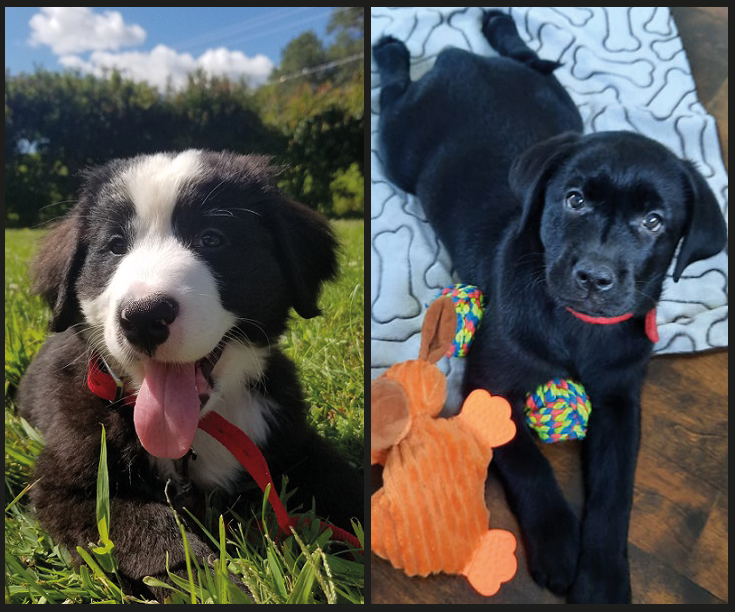
\includegraphics{images/ImageCouverture.png}\\[\bigskipamount]

}
\posttitle{
\end{center}
}


%\let\oldmaketitle\maketitle
%\AtBeginDocument{\let\maketitle\relax}

